\tikzstyle{document} = [circle, rounded corners ,text centered, draw=black]
\tikzstyle{topic} = [draw,thick,minimum width=1cm,minimum height=4cm]
\tikzstyle{tf-idf} = [draw,thick,minimum width=1cm,minimum height=1cm]

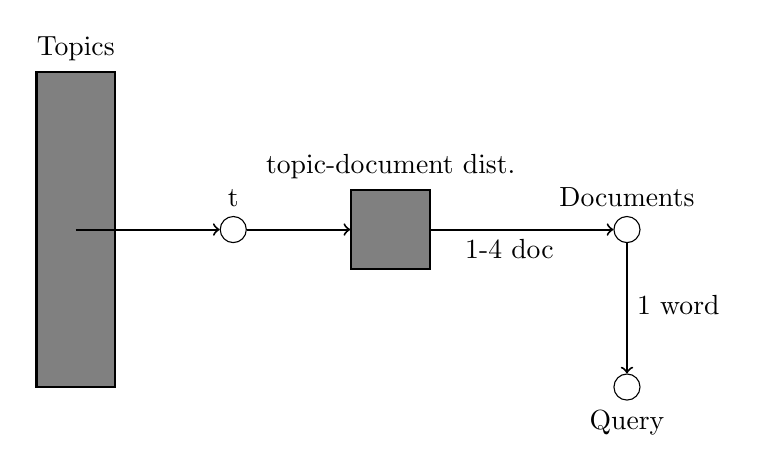
\begin{tikzpicture}
    \node [fill=gray, label={Topics}] (topic) at (0,0) [topic] {};
    \onslide<2->{
        \node [document, label={t}] (top) at (2, 0) {};
        \draw [line width=0.25mm, ->] (0,0) -> (top) node [right] {};
    };
    \onslide<3->{
        \node [fill=gray, label={topic-document dist.}] (dist) at (4,0) [tf-idf] {};
        \draw [line width=0.25mm, ->] (top) -> (dist)  {};
    };
    \onslide<4->{
        \node [document, label={Documents}] (documents) at  (7, 0) {};
        \draw [line width=0.25mm, ->] (dist) -- node[below] {1-4 doc} ++(2.5,0) -- (documents);
    };
    \onslide<5->{
        \node [document, label=below:Query] (query) at  (7, -2) {};
        \draw [line width=0.25mm, ->] (documents) -- node[right] {1 word} ++(0,-1.75) -- (query);
    };
\end{tikzpicture}